\documentclass[aspectratio=43]{beamer}
\usepackage{hyperref}
\usepackage{graphicx}

\usepackage{amsmath}
\usepackage{amsfonts}
\usepackage{amssymb}
\usepackage{amsthm}
\usepackage{tikz}
\usepackage{xcolor}
\usepackage{array}
\usepackage{enumitem}
\usepackage{tabularx}

\usetheme{Madrid}
\usecolortheme{default}

\setbeamertemplate{navigation symbols}{}

\setbeamertemplate{footline}{}

\title{}
\author{}
\date{}

\begin{document}
\begin{frame}
\frametitle{Alternative proofs of Pascal's recurrence}

\begin{block}{Theorem}
\[
\binom{n}{k} = \binom{n-1}{k} + \binom{n-1}{k-1}
\]
\end{block}

\begin{block}{Proof \#2}
Fix an $n$-element set $S$. Select a distinguished element $s \in S$.
Each $k$-element subset of $S$ either contains $s$ or it does not.
\end{block}

\begin{block}{Proof \#3}
\begin{align*}
\binom{n-1}{k} + \binom{n-1}{k-1} &= \frac{(n-1)!}{k!(n-1-k)!} + \frac{(n-1)!}{(k-1)!(n-k)!} \\
&= \frac{(n-1)!(n-k+k)}{k!(n-k)!} = \binom{n}{k}
\end{align*}
\end{block}

\end{frame}

\begin{frame}
\frametitle{Binomial coefficients}

\begin{block}{Definition}
In the special case $j = 2$, we will use the simplified notation
\[
\binom{n}{k} \overset{\text{def}}{=} \binom{n}{k, n-k} = \frac{n!}{k!(n-k)!}.
\]
These numbers are called \textit{binomial coefficients}.
\end{block}

Binomial coefficients play important roles in many applications.

One example is \textit{binomial distributions} in probability theory.

\end{frame}

\begin{frame}
    \frametitle{Ordered set partitions}

    As before, assume that $n = n_1 + \cdots + n_j$.

    \bigskip

    \textbf{Corollary}

    The number of ways to partition an $n$-element set $S$ into disjoint subsets $S_1, \dots, S_j$ of sizes $n_1, \dots, n_j$, respectively, is $\binom{n}{n_1 \cdots n_j}$.

    \bigskip

    Important: the subsets are numbered, i.e., labeled by $1, \dots, j$. The elements within each subset are not ordered/labeled.

    \bigskip

    \textbf{Example}

    The number of ways to assign $n$ workers to $j$ different tasks requiring $n_1, \dots, n_j$ workers, respectively, is $\binom{n}{n_1 \cdots n_j}$.

    \bigskip

    \textbf{Proof}

    Such ordered set partitions are encoded by permutations of multisets.

\end{frame}

\begin{frame}
\frametitle{Pascal's recurrence}

\begin{center}
    \begin{tabular}{|c|c|c|c|c|c|c|c|}
    \hline
        1 & 4 & 10 & 20 & 35 & 56 & 84 & 120 = $\binom{10}{7}$ \\ \hline
        1 & 3 & 6 & 10 & 15 & 21 & 28 & 36 \\ \hline
        1 & 2 & 3 & 4 & 5 & 6 & 7 & 8 \\ \hline
        1 & 1 & 1 & 1 & 1 & 1 & 1 & 1 \\ \hline
    \end{tabular}
    
    A \hspace{7cm} B
\end{center}

\begin{block}{Theorem}
    \[
    \binom{n}{k} = \binom{n-1}{k} + \binom{n-1}{k-1}
    \]
\end{block}

\end{frame}

\usepackage{graphicx}
\usepackage{hyperref}

\begin{frame}
\frametitle{Pascal's Triangle}

\begin{center}
1 \\
1 \hspace{0.5cm} 1 \\
1 \hspace{0.5cm} 2 \hspace{0.5cm} 1 \\
1 \hspace{0.5cm} 3 \hspace{0.5cm} 3 \hspace{0.5cm} 1 \\
1 \hspace{0.5cm} 4 \hspace{0.5cm} 6 \hspace{0.5cm} 4 \hspace{0.5cm} 1 \\
1 \hspace{0.5cm} 5 \hspace{0.5cm} 10 \hspace{0.5cm} 10 \hspace{0.5cm} 5 \hspace{0.5cm} 1 \\
1 \hspace{0.5cm} 6 \hspace{0.5cm} 15 \hspace{0.5cm} 20 \hspace{0.5cm} 15 \hspace{0.5cm} 6 \hspace{0.5cm} 1 \\
1 \hspace{0.5cm} 7 \hspace{0.5cm} 21 \hspace{0.5cm} 35 \hspace{0.5cm} 35 \hspace{0.5cm} 21 \hspace{0.5cm} 7 \hspace{0.5cm} 1 \\
1 \hspace{0.5cm} 8 \hspace{0.5cm} 28 \hspace{0.5cm} 56 \hspace{0.5cm} 70 \hspace{0.5cm} 56 \hspace{0.5cm} 28 \hspace{0.5cm} 8 \hspace{0.5cm} 1 \\
\ldots \ldots \ldots \ldots \ldots \ldots \ldots \ldots \ldots \ldots \ldots \ldots \ldots \ldots \ldots \ldots
\end{center}

\medskip

\href{https://en.wikipedia.org/wiki/Blaise_Pascal}{\textcolor{blue}{Blaise Pascal}} (France, 1653) was the first to systematically describe
various properties of this triangle, and apply it to probability theory.

\medskip

The triangle was already known in Asia more than 1,000 years ago, thanks to \href{https://en.wikipedia.org/wiki/Pingala}{\textcolor{blue}{Halayudha}} (India), \href{https://en.wikipedia.org/wiki/Al-Karaji}{\textcolor{blue}{Al-Karaji}} (Iran), and \href{https://en.wikipedia.org/wiki/Jia_Xian}{\textcolor{blue}{Jia Xian}} (China).

\end{frame}

\begin{frame}
\frametitle{Binary strings and subsets}

\begin{block}{Corollary}
The number of binary strings of length $n$ which consist of $k$ entries equal to 1 and $n-k$ entries equal to 0 is $\binom{n}{k}$.
\end{block}

\begin{block}{Theorem}
The number of $k$-element subsets in an $n$-element set is $\binom{n}{k}$.
\end{block}

\begin{block}{Example: $n = 4$, $k = 2$}
\begin{center}
0011 \hspace{0.5cm} 0101 \hspace{0.5cm} 0110 \hspace{0.5cm} 1001 \hspace{0.5cm} 1010 \hspace{0.5cm} 1100 \\
\{C,D\} \hspace{0.3cm} \{B,D\} \hspace{0.3cm} \{B,C\} \hspace{0.3cm} \{A,D\} \hspace{0.3cm} \{A,C\} \hspace{0.3cm} \{A,B\}
\end{center}
\end{block}

\end{frame}

\begin{frame}
\frametitle{Lattice paths}

\begin{block}{Definition}
A $(NE)$ \textit{lattice path} is a sequence of points $(p_1, \dots, p_n)$ in $\mathbb{Z}^2$ such that $(p_{i+1} - p_i) \in \{(1,0), (0,1)\}$.
\end{block}

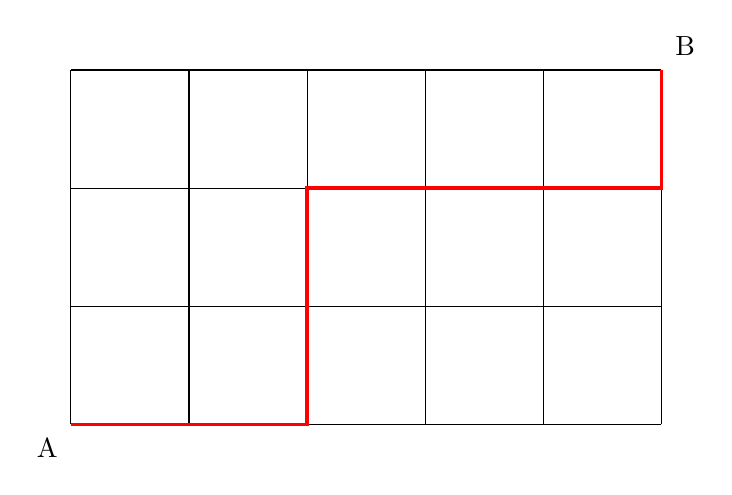
\begin{tikzpicture}[scale=1.5]
    \draw[step=1cm,color=black] (0,0) grid (5,3);
    \node at (-0.2,-0.2) {A};
    \node at (5.2,3.2) {B};
    \draw[red, very thick] (0,0) -- (2,0) -- (2,2) -- (5,2) -- (5,3);
\end{tikzpicture}

\bigskip

How many lattice paths are there from \textbf{A} to \textbf{B}?

\end{frame}

\begin{frame}
\frametitle{Compositions}

\begin{block}{Definition}
A \textit{composition} (of an integer $n$, with $k$ parts) is a positive integer solution of the equation
\begin{equation*}
    x_1 + \cdots + x_k = n. \tag{*}
\end{equation*}
A \textit{weak composition} is a nonnegative integer solution of (*).
\end{block}

\begin{block}{Example: $n=5$, $k=3$}
Compositions:
\begin{align*}
    &(3,1,1) \quad (1,3,1) \quad (1,1,3) \quad (2,2,1) \quad (2,1,2) \quad (1,2,2)
\end{align*}
Weak compositions:
\begin{align*}
    &(5,0,0) \quad (4,1,0) \quad (1,4,0) \quad (3,2,0) \quad (2,3,0) \quad (3,1,1) \quad (2,2,1) \quad (2,1,2) \\
    &(0,5,0) \quad (4,0,1) \quad (1,0,4) \quad (3,0,2) \quad (2,0,3) \quad (1,3,1) \\
    &(0,0,5) \quad (0,4,1) \quad (0,1,4) \quad (0,3,2) \quad (0,2,3) \quad (1,1,3) \quad (1,2,2)
\end{align*}
\end{block}

\end{frame}

\begin{frame}
\frametitle{Binomial identities (2)}

\begin{block}{Proposition}
\[
\binom{n}{0} + \binom{n}{1} + \cdots + \binom{n}{n} = 2^n
\]
\end{block}

\begin{center}
1 \\
1 \qquad 1 \\
1 \qquad 2 \qquad 1 \\
1 \qquad 3 \qquad 3 \qquad 1 \\
1 \qquad 4 \qquad 6 \qquad 4 \qquad 1 \\
1 \qquad 5 \qquad 10 \qquad 10 \qquad 5 \qquad 1 \\
\hrulefill
\end{center}

\begin{block}{Proof}
Count subsets of an $n$-element set, according to their size.
\end{block}

\end{frame}

\begin{frame}
\frametitle{Anagrams}

\begin{block}{Problem}
How many anagrams are there of the word STATISTICS?
\end{block}

\begin{block}{Answer}
\[
\frac{10!}{1! \cdot 1! \cdot 2! \cdot 3! \cdot 3!} = 50400.
\]
\end{block}

\begin{block}{Problem}
How many binary strings consist of three 0's and five 1's?
\end{block}

\begin{block}{Answer}
\[
\frac{8!}{3! \cdot 5!} = 56.
\]
\end{block}

\end{frame}

\begin{frame}
\frametitle{Multinomial coefficients}
\begin{block}{Theorem}
For an alphabet $\{x_1, \dots, x_j\}$ consisting of $j$ symbols, there are
\[
\binom{n}{n_1 \cdots n_j} \stackrel{\text{def}}{=} \frac{n!}{n_1! \cdots n_j!}
\]
words of length $n$ consisting of
\begin{itemize}
    \item $n_1$ copies of letter $x_1$,
    \item $\dots$,
    \item $n_j$ copies of letter $x_j$.
\end{itemize}
(Here $n = n_1 + \cdots + n_j$.)
\end{block}

\begin{block}{Proof}
Use the Division Principle: permute $n$ cards carrying those letters.
\end{block}
The numbers $\binom{n}{n_1 \cdots n_j}$ are called \textit{multinomial coefficients}.

A multinomial coefficient counts permutations of a \textit{multiset}.
\end{frame}

\begin{frame}
    \frametitle{Binomial identities (1)}

    There are many algebraic identities involving binomial coefficients.\\
    Behind each of them, there is a combinatorial correspondence.

    \vspace{0.2cm}
    To prove an identity, we either (a) ``reverse engineer'' an enumerative problem that can be solved in two different ways, or (b) establish a bijection between two sets, then enumerate each of them.

    \vspace{0.5cm}
    \begin{block}{Proposition}
        \[
            \binom{n}{k} = \binom{n}{n-k}
        \]
    \end{block}

    \vspace{0.5cm}
    \begin{block}{Proof}
        Set up a bijection between $k$-element and $(n-k)$-element subsets.
    \end{block}
\end{frame}

\begin{frame}
    \frametitle{Counting weak compositions}
    \begin{block}{Theorem}
        The number of weak compositions of $n$ with $k$ parts is equal to
        \[
        \binom{n+k-1}{k-1}.
        \]
    \end{block}
    \begin{block}{Example: $n = 2$, $k = 3$}
        \[
        \begin{array}{cccccc}
            (2,0,0) & (0,2,0) & (0,0,2) & (1,1,0) & (1,0,1) & (0, 1, 1) \\
            \circ \circ || & | \circ \circ | & || \circ \circ & \circ | \circ | & \circ || \circ & | \circ | \circ \\
            0011 & 1001 & 1100 & 0101 & 0110 & 1010
        \end{array}
        \]
    \end{block}
\end{frame}

\begin{frame}
\begin{center}
Math 465: Introduction to Combinatorics

\bigskip
\bigskip

Andrew Sack

\bigskip
\bigskip
\bigskip
\bigskip

Quiz \#1: 30 minutes, 5 questions, open Friday--Saturday.

Homework \#1: due Monday evening.

These slides will be posted on Canvas.
\end{center}
\end{frame}

\begin{frame}
\frametitle{Counting words, continued}

\begin{block}{Theorem}
For an $n$-element alphabet, there are
\[ (n)_k \overset{\text{def}}{=} n(n-1)\cdots (n - k + 1) = \frac{n!}{(n-k)!} \]
words of length $k$ without repetitions.
\end{block}

These numbers are called \textit{falling powers}.

\begin{block}{Proof 1}
Use the Multiplication Principle.
\end{block}

\begin{block}{Proof 2}
Use the Division Principle: take a permutation of the alphabet, then
remove the last $n - k$ symbols.
\end{block}

\end{frame}

\begin{frame}
\frametitle{Counting compositions}

\begin{block}{Theorem}
The number of compositions of $n$ with $k$ parts is equal to $ \binom{n-1}{k-1} $.
\end{block}

\begin{block}{Proof}
\centering
$\left\{ \begin{array}{c} \text{compositions of } n \\ \text{with } k \text{ parts} \end{array} \right\} \longleftrightarrow \left\{ \begin{array}{c} \text{weak compositions of } n - k \\ \text{with } k \text{ parts} \end{array} \right\} $

\vspace{0.2cm}
Example: $n = 5$, $k = 3$

$(3,1,1) \quad (1,3,1) \quad (1,1,3) \quad (2,2,1) \quad (2,1,2) \quad (1,2,2)$

$(2,0,0) \quad (0,2,0) \quad (0,0,2) \quad (1,1,0) \quad (1,0,1) \quad (0,1,1)$

\vspace{0.2cm}
The number of these weak compositions is $ \binom{(n-k)+k-1}{k-1} = \binom{n-1}{k-1}$.
\end{block}

\end{frame}

\begin{frame}
    \frametitle{Binomial identities (3)}

    \begin{block}{Proposition}
        For $n \geq 1$, we have $\binom{n}{0} - \binom{n}{1} + \cdots + (-1)^n \binom{n}{n} = 0$.
    \end{block}

    \vspace{0.5cm}
    
    \begin{center}
    1 \\
    1 \hspace{0.5cm} 1 \\
    1 \hspace{0.5cm} 2 \hspace{0.5cm} 1 \\
    1 \hspace{0.5cm} 3 \hspace{0.5cm} 3 \hspace{0.5cm} 1 \\
    1 \hspace{0.5cm} 4 \hspace{0.5cm} 6 \hspace{0.5cm} 4 \hspace{0.5cm} 1 \\
    1 \hspace{0.5cm} 5 \hspace{0.5cm} 10 \hspace{0.5cm} 10 \hspace{0.5cm} 5 \hspace{0.5cm} 1
    \end{center}

    \vspace{0.5cm}

    \begin{block}{Proof}
        Get a bijection between subsets of even and odd size, by matching each subset containing a fixed element $s$ to a subset not containing $s$.
    \end{block}

\end{frame}

\begin{frame}
\frametitle{Binomial identities (4)}

\begin{block}{Theorem}
\[
\sum_{k} \binom{n}{k} \binom{m}{\ell - k} = \binom{n + m}{\ell}
\]
\end{block}

\begin{block}{Proof}
Consider a disjoint union of two sets of sizes $n$ and $m$, respectively.  
Then count the $\ell$-element subsets of this union.

\vspace{0.5cm}

\begin{center}
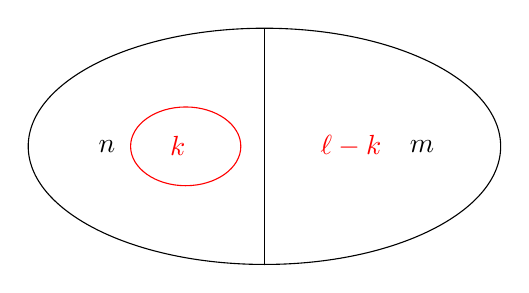
\begin{tikzpicture}
  \draw (0,0) ellipse (3cm and 1.5cm);
  \draw (0,0) -- (0,1.5);
  \draw (0,0) -- (0,-1.5);
  \draw[red] (-1,0) ellipse (0.7cm and 0.5cm);
  \node at (-2,0) {$n$};
  \node[red] at (-1.1,0) {$k$};
  \node[red] at (1.1,0) {$\ell - k$};
  \node at (2,0) {$m$};
\end{tikzpicture}
\end{center}

\end{block}

\end{frame}

\begin{frame}
\frametitle{Binomial identities (7)}

\begin{block}{Proof \#2 of the identity $\sum_{k=0}^{n} \binom{n}{k}^2 = \binom{2n}{n}$}
The number of \textit{lattice paths} from $\mathbf{A} = (0,0)$ to $\mathbf{B} = (n, n)$ equals $\binom{2n}{n}$.
For each of these paths, look where it crosses \textcolor{cyan}{the diagonal}.
\end{block}

\begin{center}
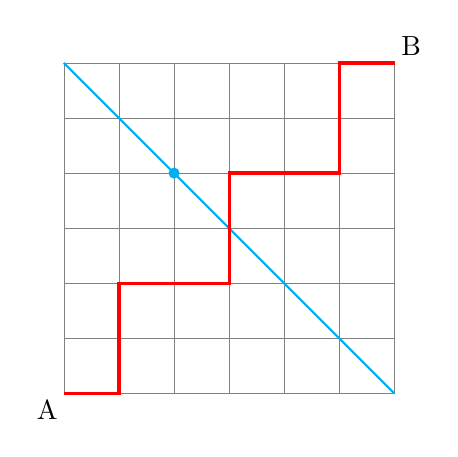
\begin{tikzpicture}[scale=0.7]
\draw[step=1,gray,very thin] (0,0) grid (6,6);
\draw[cyan, thick] (0,6) -- (6,0);
\fill[cyan] (2,4) circle (0.1);
\node at (-0.3,-0.3) {A};
\node at (6.3,6.3) {B};
\draw[red, very thick] (0,0) -- (1,0) -- (1,2) -- (3,2) -- (3,4) -- (5,4) -- (5,6) -- (6,6);
\end{tikzpicture}
\end{center}

\end{frame}

\begin{frame}
\frametitle{Binomial identities (6)}
\begin{block}{Example}
\[1^2 + 4^2 + 6^2 + 4^2 + 1^2 = 70 = \binom{8}{4}\]
\end{block}

\begin{center}
\begin{tabular}{ccccccccccccccccc}
                 &                  &                  &                  &                  &                  &                  &        1         &                  &                  &                  &                  &                  &                  &         \\
                 &                  &                  &                  &                  &                  &                  &  1          &                  1 &                  &                  &                  &                  &                  &         \\
                 &                  &                  &                  &                  &                  &      1           &                  &  2          &                  &  1          &                  &                  &                  &         \\
                 &                  &                  &                  &                  &      1           &                  & 3           &                  &  3          &                  &  1          &                  &                  &         \\
                 &                  &                  &                  &       1          &                  & 4           &                  &  6          &                  &  4          &                  &  1          &                  &         \\
                 &                  &                  &      1           &                  &  5          &                  & 10           &                  & 10          &                  &  5          &                  &  1          &         \\
                 &                  &      1           &                  &  6          &                  &  15           &                  & 20          &                  & 15          &                  &  6          &                  &  1         \\
                 &      1           &                  &  7          &                  &  21           &                  & 35          &                  & 35          &                  & 21          &                  &  7          &                  &   1     \\
    1            &                  &  8          &                  &  28           &                  & 56          &                  & 70          &                  & 56          &                  & 28          &                  &  8          &         1 \\
\end{tabular}

\hrulefill
\end{center}

\end{frame}

\begin{frame}
\frametitle{Counting lattice paths using the Addition Principle}

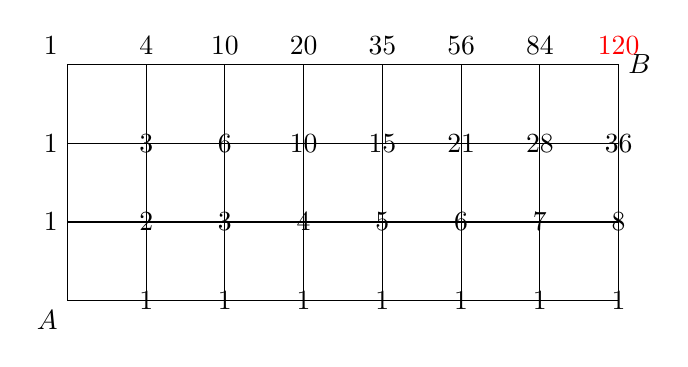
\begin{tikzpicture}
  % Define grid coordinates
  \foreach \x in {0,1,2,3,4,5,6,7}
    \foreach \y in {0,1,2,3}
      \coordinate (P\x\y) at (\x,\y);

  % Draw grid lines
  \foreach \x in {0,1,2,3,4,5,6,7}
  {
    \draw (P\x0) -- (P\x3);
  }
  \foreach \y in {0,1,2,3}
  {
    \draw (P0\y) -- (P7\y);
  }

  % Add numbers
  \node at (P03) [above left] {$1$};
  \node at (P13) [above] {$4$};
  \node at (P23) [above] {$10$};
  \node at (P33) [above] {$20$};
  \node at (P43) [above] {$35$};
  \node at (P53) [above] {$56$};
  \node at (P63) [above] {$84$};
  \node at (P73) [above, color=red] {$120$};

  \node at (P02) [left] {$1$};
  \node at (P12) {$3$};
  \node at (P22) {$6$};
  \node at (P32) {$10$};
  \node at (P42) {$15$};
  \node at (P52) {$21$};
  \node at (P62) {$28$};
  \node at (P72) {$36$};

  \node at (P01) [left] {$1$};
  \node at (P11) {$2$};
  \node at (P21) {$3$};
  \node at (P31) {$4$};
  \node at (P41) {$5$};
  \node at (P51) {$6$};
  \node at (P61) {$7$};
  \node at (P71) {$8$};

  \node at (P00) [below left] {$A$};
  \node at (P10) {$1$};
  \node at (P20) {$1$};
  \node at (P30) {$1$};
  \node at (P40) {$1$};
  \node at (P50) {$1$};
  \node at (P60) {$1$};
  \node at (P70) {$1$};
  \node at (P73) [right] {$B$};
\end{tikzpicture}

\end{frame}

\begin{frame}
\frametitle{Lattice paths and binomial coefficients}

\begin{block}{Theorem}
The number of lattice paths from $(0,0)$ to $(k, \ell)$ is equal to $\binom{k+\ell}{k}$.
\end{block}

\begin{block}{Proof}
Such lattice paths are in bijection with the binary strings containing $k$ entries equal to 1 and $\ell$ entries equal to 0 (or with $k$-element subsets of a $(k + \ell)$-element set).
\end{block}

\begin{center}
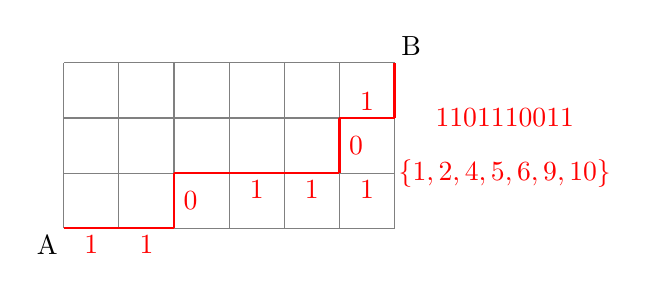
\begin{tikzpicture}[scale=0.7]
\draw[step=1cm,gray,thin] (0,0) grid (6,3);
\node at (-0.3,-0.3) {A};
\node at (6.3,3.3) {B};

\draw[red, thick] (0,0) -- (1,0);
\draw[red, thick] (1,0) -- (2,0);
\draw[red, thick] (2,0) -- (2,1);
\draw[red, thick] (2,1) -- (3,1);
\draw[red, thick] (3,1) -- (4,1);
\draw[red, thick] (4,1) -- (5,1);
\draw[red, thick] (5,1) -- (5,2);
\draw[red, thick] (5,2) -- (6,2);
\draw[red, thick] (6,2) -- (6,3);

\node[red] at (0.5, -0.3) {1};
\node[red] at (1.5, -0.3) {1};
\node[red] at (2.3, 0.5) {0};
\node[red] at (3.5, 0.7) {1};
\node[red] at (4.5, 0.7) {1};
\node[red] at (5.5, 0.7) {1};
\node[red] at (5.3, 1.5) {0};
\node[red] at (5.5, 2.3) {1};

\node[red] at (8, 2) {$1101110011$};
\node[red] at (8, 1) {$\{1, 2, 4, 5, 6, 9, 10\}$};
\end{tikzpicture}
\end{center}

\end{frame}

\begin{frame}
\frametitle{Binomial identities (5)}

\begin{block}{Corollary}
\[
\sum_{k=0}^{n} \binom{n}{k}^2 = \binom{2n}{n}
\]
\end{block}

\begin{block}{Proof \#1}
Apply the identity
\[
\sum_{k} \binom{n}{k} \binom{m}{\ell - k} = \binom{n+m}{\ell}
\]
with $\ell = m = n$, and use that $\binom{n}{n-k} = \binom{n}{k}$.
\end{block}

\end{frame}
\end{document}